\subsection{Back-end}

\hspace{0.5cm} Połączenia z serwerami DNS będą realizowane za pomocą oprogramowania OpenVPN. Na początku pierwszy proces w Pythonie inicjuje połączenie VPN i tworzy dla niego sieciową przestrzeń nazw. Następnie w tej przestrzeni jest uruchamiany drugi proces, który zbiera informację o połączeniu i przesyła je do bazy danych. Po zakończeniu tego procesu przestrzeń nazw jest usuwana, a połączenie VPN zakończone. Te czynności są następnie powtarzane dla wszystkich pozostałych połączeń. 

Poniżej przedstawiony jest schemat tej operacji: 
\\~\\
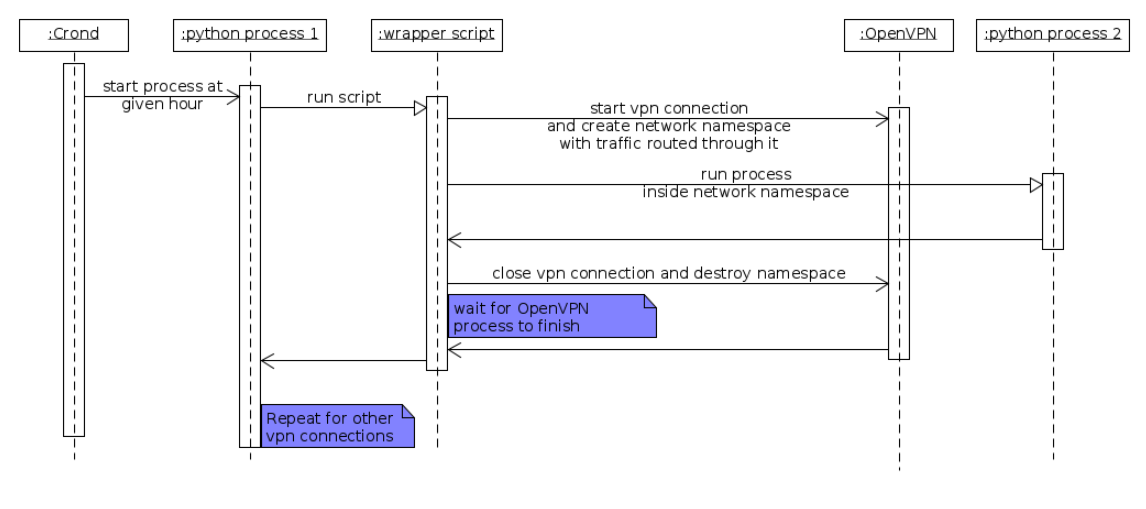
\includegraphics[scale=0.65]{connection_schema.png}
